\subsection{Baselines}
\label{subsection:baseline}

	En esta sección se detallan los experimentos y los resultados obtenidos de realizar una reimplementación del trabajo de Wang et. al. en \cite{wang}. El objetivo es definir el baseline para el resto de los experimentos con imágenes reales y sintéticas. Así también, se definen los parámetros comunes a todos los experimentos como la configuración de HOG, $\alpha$, parámetro de i\-ni\-cia\-li\-za\-ción de las tablas, entre otros.
	
	Posteriormente se van a mostrar y explicar los resultados de los experimentos con imágenes reales. Se detalla el impacto de los diferentes esquemas de binarización con el fin de seleccionar el más adecuado para el resto de los experimentos.
	
	
\subsubsection{Reimplementación de Wang et. al.}

	En este experimento se utilizan, para el entrenamiento del clasificador, solamente imágenes de caracteres segmentados de escenas naturales e i\-má\-ge\-nes sintéticas, ver \ref{subsection:evaluacion}, siguiendo lo detallado por Wang et. al. en \cite{wang}. La e\-va\-lua\-ción del clasificador se realiza sobre un conjunto de prueba proporcionado por el dataset \textit{Chars74k-15} y se mantiene fijo durante todos los experimentos del presente trabajo.
	
	De la implementación de los autores, se pudieron obtener los siguientes parámetros para los experimentos:
	\begin{itemize}
		\item \textbf{Cantidad de grupos} ($M$): $256$.
		\item \textbf{Bits por grupo} (\textit{bpg}): $6$.
	\end{itemize}
	
	Estos dos valores generan vectores de características de longitud 1536.
	
	Para la función HOG,	 se utilizan dos parámetros, la cantidad de \textit{o\-rien\-ta\-cio\-nes} y la cantidad de \textit{celdas por bloque}. En los experimentos realizados, se prueban los siguientes conjuntos de valores:
	
	\begin{itemize}
		\item Orientaciones: $\textit{o} \in \{8, 9\}$
		\item Celdas por bloque: $\textit{cpb} \in \{4, 9\}$
	\end{itemize}
	
	En cuanto al método para binarizar los descriptores HOG, luego de haber leído la implementación provista por los autores, se establece como método la generación de variables aleatorias uniformes. Este enfoque, resultó ser el más adecuado debido a que es el que más se asemeja a lo que hicieron los autores en \cite{wang}	.
	
	Finalmente, el valor $\alpha$ para la inicialización de las tablas es un parámetro que no está especificado pero es necesario para poder entrenar el clasificador. En este experimento se probaron los siguientes valores de $\alpha$ con el fin de establecer el mejor valor.
	
	\begin{itemize}
		\item $\alpha \in \{0,01; 0,1; 1\}$.
	\end{itemize}
	
	Teniendo en cuenta estos parámetros, se obtuvieron los resultados que se pueden apreciar en el cuadro \ref{table: Baseline-Table}. En la misma, expresamos como ``NATIVE+FERNS'' a los resultados obtenidos al haber entrenado y evaluado el clasificador Random Ferns con imágenes reales. De la misma ma\-ne\-ra, ``SYNTH+FERNS'' se  refiere a los experimentos donde se usaron $1000$ imágenes sintéticas durante el entrenamiento.

	\begin{table}
		\centering
	    \begin{tabular}{ | l | l | l | p{5cm} |}
    			\hline
    				\textbf{Implementación} & \textbf{Score} \\ \hline
    				Wang NATIVE+FERNS & 54\% \\ \hline
    				Impl. propia NATIVE+FERNS & 50\% \\ \hline
    				Wang SYNTH+FERNS & 47\% \\ \hline
    				Impl. propia SYNTH+FERNS & 43\% \\

    			\hline
    		\end{tabular}
    		\caption[Resultados reales y sintéticas para baseline]{Resultados obtenidos en la reimplementación del trabajo de Wang et al.}
    		\label{table: Baseline-Table}
	\end{table}

	Como se puede ver en base a los resultados expuestos en el cuadro \ref{table: Baseline-Table}, hay diferencias significativas entre los resultados de ambas implementaciones que se deben a varios factores. Existen ciertos parámetros que no están especificados en el trabajo de Wang et al. y que se detallan a continuación:
	
	\begin{itemize}
		\item \textbf{Método de binarización}: El hecho de que en la reimplementación se utilizó un lenguaje diferente, en este caso se usó Python, genera ciertos problemas. El uso de funciones que generan valores numéricos aleatorios depende mucho de la implementación de dichas funciones. Estas pueden variar entre los lenguajes por lo cual los resultados obtenidos son diferentes. La binarización hace uso de valores aleatorios con lo que se generan estas diferencias.
		\item \textbf{$\alpha$}: es el parámetro para la inicialización de las tablas que influye en la performance.
		\item \textbf{Implementación de HOG}: la implementación de HOG que usan los autores es la desarrollada por Piotr Dollár, \cite{PiotrD}, la cual es una variación del método original propuesto por Dalal \& Triggs en \cite{DT05}. En la reimplementación se utiliza la función HOG extraída de la librería de python scikit-images, que también está basada en \cite{DT05} pero difiere de la usada por los autores. Una de las diferencias entre ambas funciones está en que la desarrollada por Piotr Dollar acepta imágenes a color y la que se usa en este trabajo sólo acepta imágenes en escala de grises. Otra diferencia entre estas implementaciones está en la longitud del vector resultante. Usando los mismos parámetros en ambas funciones, la desarrollada por Piotr Dollar devuelve vectores con una longitud $4$ veces mayor a los devueltos por la función HOG usada en el presente trabajo. Esto se debe a que usa un esquema diferente de normalización.
	\end{itemize}
	
	Ante esta situación se decide por establecer como baselines los resultados obtenidos por la configuración más cercana a la usada en \cite{wang}. Teniendo en cuenta los parámetros conocidos, se establece además las siguiente configuración:
	
	\begin{itemize}
		\item \textbf{HOG}: se consideran $8$ orientaciones y $9$ celdas por bloque como los parámetros que mejores resultados produjeron.
		\item \textbf{$\alpha$}: se establece en $0.01$ pues es el valor que más impacto positivo produjo en estos experimentos.
	\end{itemize}		
	
	El esquema de binarización utilizado en este experimento sirve solamente para establecer el baseline para el resto de los experimentos. En la siguiente subsección se evalúan, a través de experimentos con imágenes reales, nuevos métodos de binarización, explicados en \ref{subsubsection:binarizacion}, y se va a considerar como baseline el valor $0.50$. De la misma manera, en la sección de los experimentos con imágenes sintéticas, el baseline pasará a ser $0.43$.
	
\subsubsection{Evaluación de Esquemas de Binarización}
\label{subsubsection: eval_esquemas}


	Esta subsección tiene como objetivo evaluar los 4 esquemas de binarización detallados en \ref{subsubsection:binarizacion}. Además, como resultado de los experimentos, se establecerá cúal es el tamaño óptimo para los grupos o \textit{ferns} y cúal es la mejor dimensión para los vectores de características. Para esto, se entrena y evalua al clasificador \textit{Random Ferns} con imágenes reales de la misma manera que en la subsección anterior.
	
	Inicialmente, se van a mostrar $4$ gráficos, que corresponden a los métodos utilizados en la binarización. Con esto se busca ver qué método devuelve los mejores resultados. Estas figuras, reflejan la diferencia en performance al considerar grupos de diferente dimensión $B/G \in \{ 1, 4, 8, 10\}$. Con esto se busca establecer, para cada caso, qué dimensión arroja los mejores resultados. Cabe aclarar que cada gráfico refleja la media de los resultados de 5 corridas del experimento junto con las barras de error a 1 desviación estándar. La Figura \ref{fig: Reales-Comparativa metodos} reúne los mejores resultados de clasificación de las primeras cuatro figuras para establecer una comparación más precisa. En la tabla \ref{table: reales-comparativa} se muestra un resumen de los mejores valores.

	 Dada la gran cantidad de parámetros que se manejan en estos experimentos, se va a dejar detallado en el análisis cuales son los mejores y se los va a usar para los siguientes experimentos.

			\begin{figure}[htbp!]
				\centering
				\centerline{
					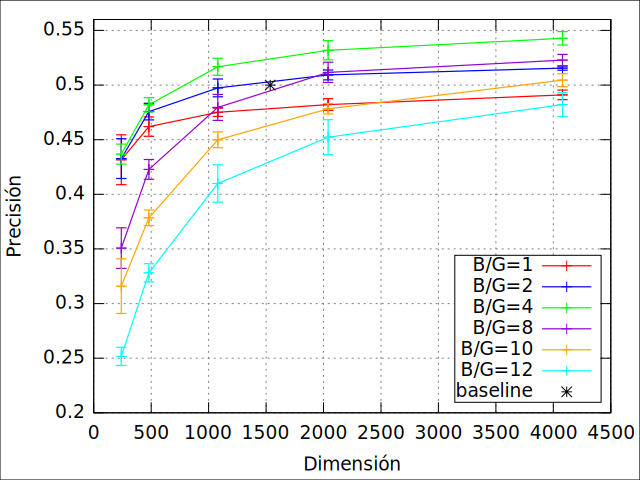
\includegraphics[scale=0.6]{img/resultados/reales/mean.png}
				}
				\caption[Resultados media]{Resultados usando la media}
				\label{fig: Reales-media}
			\end{figure}
			\begin{figure}[htbp!]
				\centering
				\centerline{
					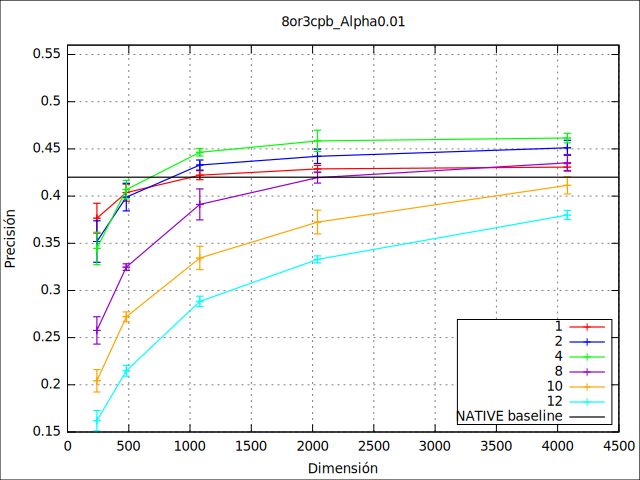
\includegraphics[scale=0.6]{img/resultados/reales/median.png}
				}
				\caption[Resultados mediana]{Resultados usando la mediana}
				\label{fig: Reales-mediana}
			\end{figure}
			\begin{figure}[htbp!]
				\centering
				\centerline{
					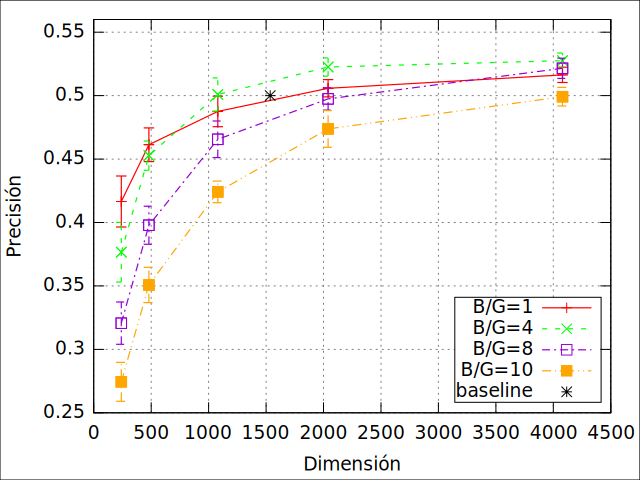
\includegraphics[scale=0.6]{img/resultados/reales/expon.png}
				}
				\caption[Resultados expon]{Resultados usando la distribución exponencial}
				\label{fig: Reales-expon}
			\end{figure}
			\begin{figure}[htbp!]
				\centering
				\centerline{
					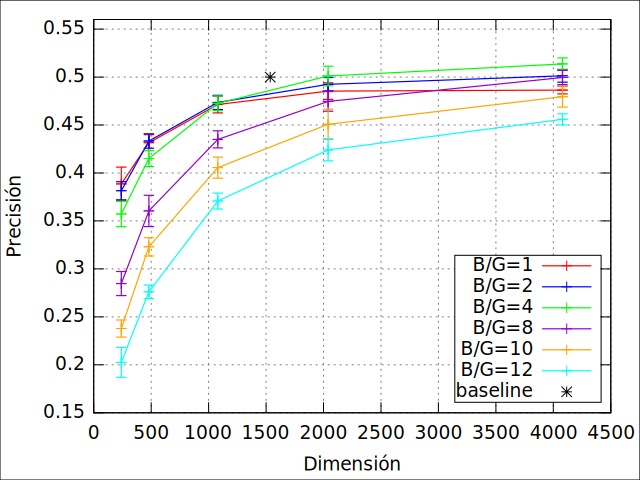
\includegraphics[scale=0.6]{img/resultados/reales/bootstrap.png}
				}
				\caption[Resultados bootstrap]{Resultados usando bootstrap}
				\label{fig: Reales-bootstrap}
			\end{figure}

	Teniendo en cuenta los resultados de los primeros $4$ gráficos, a simple vista se puede observar que los resultados obtenidos usando la media como método para binarizar los vectores son los mejores, llegando estos a un máximo cercano al $55\%$ de precisión. En el caso opuesto, el usar la mediana arrojó los peores resultados, ya que, en el mejor de los casos, se supera el $47\%$ a diferencia de bootstrap que llega a $51\%$ . El uso de la distribución exponencial en los casos donde la longitud de los grupos es baja, $1$ bit por grupo, no supera a la media en performance pero aumenta a medida que aumentamos este valor, casos $\{ 4, 8, 10\}$ bits por grupo. Los valores que podemos encontrar en \ref{fig: Reales-expon} se acercan a los de la media llegando a un máximo en la precisión de $53\%$. En cuanto al uso de bootstrap, se puede apreciar que los resultados se mantienen por debajo de los obtenidos con la distribución exponencial y la media con valores que rondan entre $45\%$ y $52\%$, en el mejor de los casos.

	En cuanto a las dimensiones del vector binario evaluadas en el ex\-pe\-ri\-men\-to $\{ 240, 480, 1080, 2040, 4080 \}$, es claro que a medida que aumentamos la longitud de los vectores aumenta la performance. Se puede ver que, cuando se usan vectores de longitud reducida, en este caso $240$, se marca una diferencia importante en la precisión entre los experimentos realizados con grupos de dimensionalidad baja $\{ 1, 4 \}$ y alta $\{8, 10\}$. Es decir, dejando fija la dimensión de los vectores en $240$, mientras más chico es el tamaño de los grupos mejor es el resultado, se puede observar en cualquiera de las figuras. En el otro extremo, si usamos grupos de $10$ bits la precisión disminuye considerablemente. La misma relación se mantiene a medida que aumentamos el tamaño de los vectores de características hasta cierto punto. Por ejemplo, en la Figura \ref{fig: Reales-media} es claro que a partir del uso de $1080$ como tamaño de vector en adelante, el uso de grupos de longitud mayor arroja mejores resultados. Lo mismo sucede en las otras figuras en diferentes puntos.

	En cuanto al uso del valor $4080$, se puede ver que no hay un aumento considerable en la performance que lo diferencie del uso de $2040$. Con esto en mente, es conveniente hacer uso de este último valor ya que usa vectores mucho más chicos incrementando la eficiencia en el cómputo.

	El enfoque del clasificador Ferns es semi-na\"{i}ve, es decir, a diferencia del clasificador Na\"{i}ve Bayes, se considera que hay cierta relación de dependencia o correlación entre las dimensiones del vector de características. Por lo tanto, tal y como se explica en \ref{subsection:ferns}, los vectores se dividen en grupos de dimensión \textit{S}. Esto con el objetivo de ir un paso más allá de la independencia propuesta en Na\"{i}ve Bayes donde cada dimensión es independiente y así poder capturar estas correlaciones. El problema con los vectores binarizados de dimensión reducida, es que almacenan menos información sobre los datos de la imagen a comparación de los vectores cuya longitud es mayor. En cada grupo, se capturan las correlaciones entre las dimensiones involucradas en estos, es decir, el nivel de dependencia o relación que existen entre las mismas. Es por eso que al aumentar la dimensionalidad de los vectores en el proceso de binarización, capturamos más estructuras de correlación de los datos. Basándonos en esto, y como se puede observar en los gráficos expuestos, los grupos de $4$ bits son los más adecuados en la clasificación en la mayoría de los casos.

			\begin{figure}[htbp]
				\centering
				\centerline{
					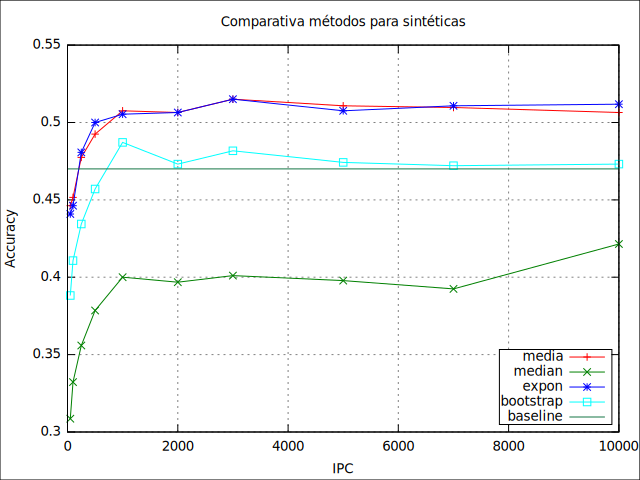
\includegraphics[scale=0.6]{img/resultados/reales/comparativa_metodos.png}
				}
				\caption[Reales comparativa]{El gráfico muestra las mejores curvas de los gráficos presentados con la mejor configuración}
				\label{fig: Reales-Comparativa metodos}
			\end{figure}

	Del análisis realizado surge que la mejor configuración está dada por: \textit{bits por grupo = $4$} y \textit{dimensión del vector = $2040$}. Se puede observar en la Figura \ref{fig: Reales-Comparativa metodos} las mejores curvas para cada método, utilizando la mejor configuración, a excepción de la longitud del vector con el objetivo de ver la curva de crecimiento. Queda claro que la media se puede establecer como el mejor método para la binarización por lo que en los próximos experimentos se procederá a trabajar con este método de binarización. La diferencia en precisión entre usar vectores de longitud $2040$ y $4080$ no es notable en los $4$ casos por lo cual como dijimos anteriormente, el uso de $2040$ dimensiones permite ob\-te\-ner buenos resultados con un menor costo computacional. En todos los casos, salvo cuando se usa la mediana como método de binarización, se supera el baseline propuesto en diferentes puntos. La media logra una diferencia de $4\%$ con respecto al baseline pero usando vectores de dimensión $4080$, la misma diferencia baja a un $3\%$ si consideramos $2040$.

	La tabla \ref{table: reales-comparativa} muestra un resumen de los valores obtenidos con la mejor configuración para cada método.

	\begin{table}
		\centering
		\begin{tabular}{ | l | l | l | p{5cm} |}
    			\hline
    				\textbf{NATIVE + FERNS} & \textbf{Score} \\ \hline
    				Media & 53\% \\ \hline
    				Mediana & 46\%\\ \hline
    				Exponencial & 52\% \\ \hline
    				Bootstrap & 50\%\\
    			\hline
    		\end{tabular}
    		\caption[Resultados imágenes naturales]{Tabla comparativa entre los diferentes métodos propuestos para la binarización en la clasificación de caracteres en escenas naturales usando la mejor configuración de parámetros.}
    		\label{table: reales-comparativa}
    	\end{table}





	